\section{Unscented Kalman Filter}
\label{unscented_kalman_filter}

In the previous section, we saw how linearization errors can cause the EKF to produce state estimates that are very different from
the true value of the state and produce covariances that don't accurately
capture the uncertainty in the state. This can be a big problem when we're relying on the EKF in safety critical applications
like self driving cars. In this section, we will discuss the Unscented Kalman
Filter, which is an alternative approach to nonlinear Kalman filtering that
relies on something called the unscented transform to pass probability
distributions through nonlinear functions. As we will see, the unscented transform
gives us much higher accuracy than analytical EKF style linearization,
for a similar amount of computation, and without needing to compute any Jacobians. 

Hence, by the end of this section, you will be able to use the unscented transform to pass a probability distribution
through a nonlinear function. Describe how the Unscented Kalman Filter, or UKF, uses the unscented transform in
the predication and correction steps. And explain the advantages
of the UKF over the EKF, as well as apply the UKF to a simple
nonlinear tracking problem. 

\section{The unscented transform}
\label{unscented_transform}

The intuition behind the unscented
transform is simple. It's typically much easier to approximate a probability distribution than it is to approximate an arbitrary
nonlinear functions. Let's see  a simple example where a 1D Gaussian distribution like the one on shown on Figure, gets transforms
to a nonlinear function into a more complicated a 1D distribution
like the one on the right. 

\begin{figure}[!htb]
\begin{center}
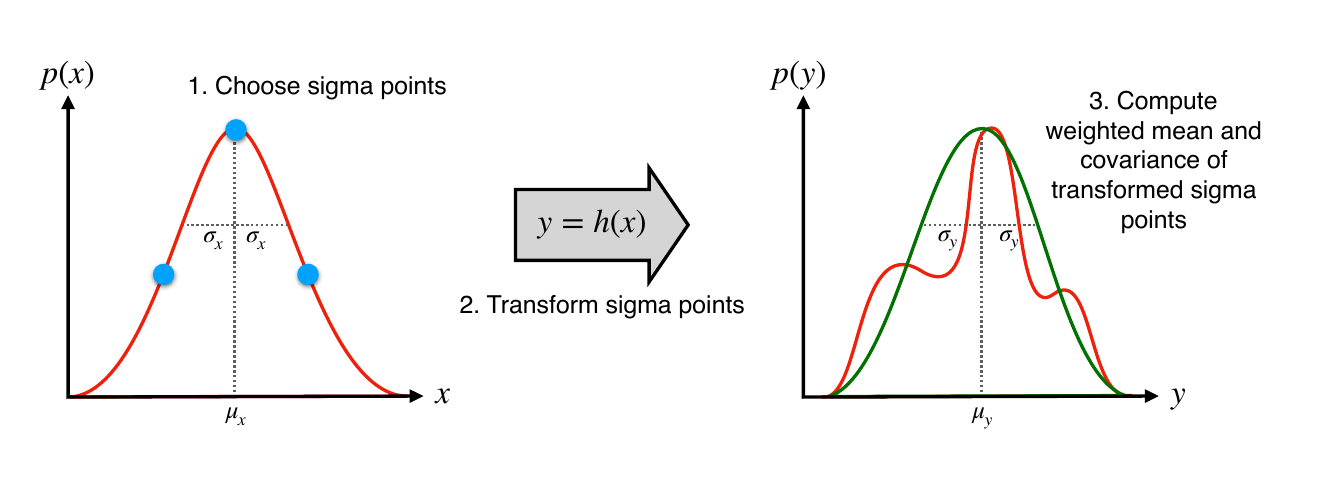
\includegraphics[scale=0.280]{img/unscented_kalman_filter/unscented_kalman_filter_1.jpeg}
\end{center}
\caption{Summary of EKF.}
\label{unscented_kalman_filter_1}
\end{figure}

We already know the mean and standard deviation of the input Gaussian, and we want to figure out the mean and
standard deviation of the output distribution using this information and
the nonlinear function. The unscented transform
gives us a way to do this. The basic idea in the unscented
transform has three steps. 

\begin{itemize}
\item We choose a set of sample points from our input distribution. These are not random samples,
they are deterministic samples, chosen to be a certain number of standard deviations away from the mean. For this reason,
these samples are called sigma points and the unscented transform is sometimes
called the sigma point transform. 
\item Once we have our set of carefully chosen sigma points, the second and easiest step is to pass each sigma point
to our nonlinear function producing a new set of sigma points belonging to the output distribution. 
\item Finally, we can compute the sample mean and covariance of the output sigma points with some carefully chosen weights, and
these will give us a good approximation of the mean and covariance of the true output distribution. 
\end{itemize}

Now, that we have seen the basic
idea of the unscented transform, let's look at each of these steps in detail. 

The first thing you might be wondering is, how many sigma points do we need and which points are in fact sigma points? In general, for
an $N$-dimensional probability distribution $N(\mu, \Sigma)$, we need $2N + 1$ sigma points. One for the mean, and the rest
symmetrically distributed about the mean. The diagrams on the left show the sigma
points for one dimensional and two dimensional examples. 

\begin{figure}[!htb]
\begin{center}
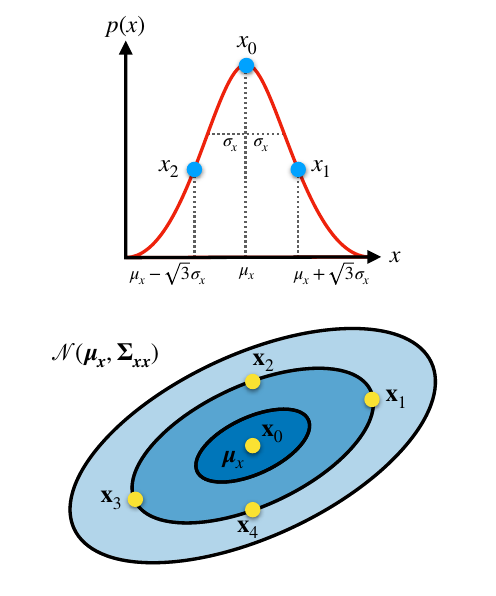
\includegraphics[scale=0.280]{img/unscented_kalman_filter/unscented_kalman_filter_2.jpeg}
\end{center}
\caption{Summary of EKF.}
\label{unscented_kalman_filter_2}
\end{figure}

In 1D, we need two sigma points, and in 2D, we need five. The first step in determining where
the sigma point is taking something called the Cholesky decomposition
of the covariance matrix associated with the input distribution. The Cholesky decomposition is basically
a square root operation that operates on symmetric positive definite matrices,
such as covariance matrices. 


\begin{equation}
\Sigma = LL^T
\end{equation}

where $L$ is a lower triangular matrix.

\begin{framed}
\theoremstyle{remark}
\begin{remark}{\textbf{Cholesky Decomposition}}

\end{remark}
\end{framed}

In fact, if the input PDF is one dimensional, the Cholesky decomposition really is
just the square root of the variance which is also known as
the standard deviation. We will not go into the details of how
to compute a Cholesky decomposition. 

Once we have decomposed the covariance matrix, we can choose our first sigma point to
be the mean of the distribution and the remainder to be the mean plus or
minus some factor times each column of the matrix $L$ that
we got from the Cholesky decomposition. 

\begin{eqnarray}
\mathbf{x}_0 = \boldsymbol{\mu} \\
\mathbf{x}_i = \boldsymbol{\mu} + \sqrt{N + \kappa} \text{col}_i L, ~~ i = 1, \ldots, L
\end{eqnarray}

The value of $N$ here again is the number of dimensions of the probability distribution. The parameter $\kappa$ is a tuning parameter
that you're free to set yourself. For Gaussian distributions, which is what we will be working with, setting $N + \kappa$ equal
to three is a good choice. 

\begin{eqnarray}
\mathbf{x}_{i + N} = \boldsymbol{\mu} - \sqrt{N + \kappa} \text{col}_i L, ~~ i = 1, \ldots, L, \kappa = 3 - N
\end{eqnarray}

So now we have our set of sigma points. The next step is straight forward, just
pass each of the sigma points through our nonlinear function $\mathbf{h}(\mathbf{x})$ to get a new
set of transform sigma points. Now all that is left is to recombine the transform sigma points to find our output mean and
output covariance. We do this using the standard formulas for the sample mean and covariance that you would have seen in you introductory statistics courses. 


\begin{eqnarray}
\boldsymbol{\mu} = \sum_{i=0}^{2N} \alpha_i \mathbf{y}_i \\
\Sigma = \sum_{i=0}^{2N} \alpha_i (\mathbf{y}_i - \boldsymbol{\mu})(\mathbf{y}_i - \boldsymbol{\mu})^T \\
\alpha_i = 
\begin{choices}
\frac{\kappa}{N + \kappa}, i =0 \\
\frac{1}{2}\frac{1}{N + \kappa}, \text{otherwise}
\end{choices}
\end{eqnarray


The trick is that each of the points gets a specific weight in the mean and covariance calculations, and that weight
depends on the parameter $\kappa$ and the dimension of the input distribution $N$. 

\section{Unscented Kalman filter example}

To see the unscented transform in action, let get back to our example
from the Extended Kalman Filter. Where we nonlinearly transformed a uniform
distribution in polar coordinates into Cartesian coordinates. Let us see how the unscented
transform compares to the analytical linearization approach. 

So here again, we have the true mean and covariance of the two
distributions in green. Now let's apply the unscented transform. 


\begin{figure}[!htb]
\begin{center}
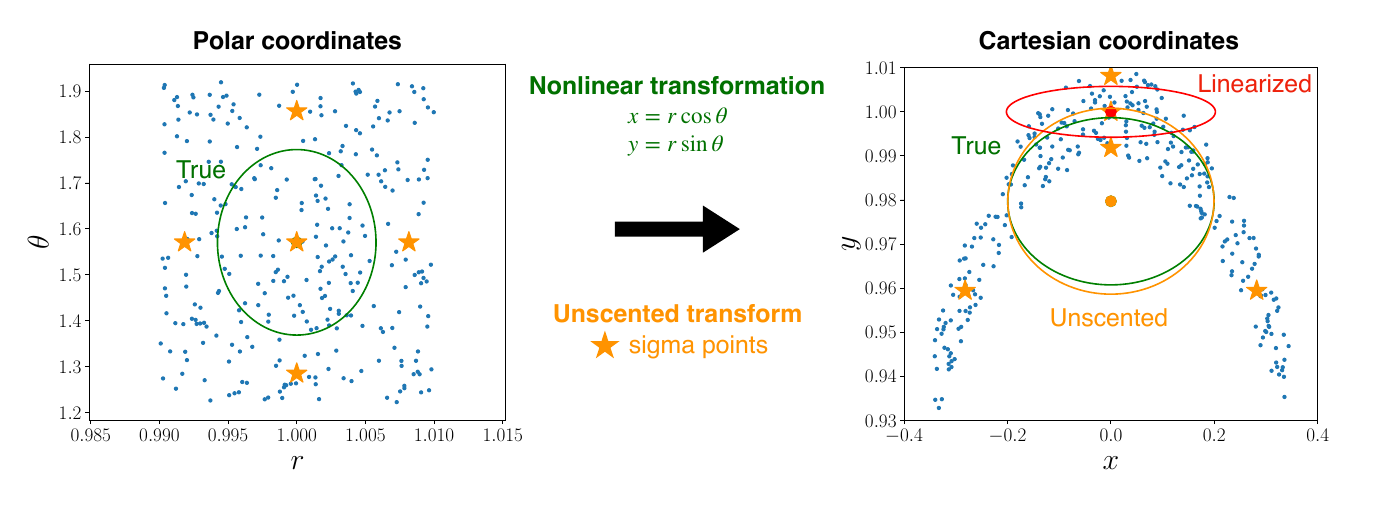
\includegraphics[scale=0.280]{img/unscented_kalman_filter/unscented_kalman_filter_3.jpeg}
\end{center}
\caption{Summary of EKF.}
\label{unscented_kalman_filter_3}
\end{figure}

The dimension of our input distribution is two so we need five sigma points which
we have shown as orange stars. Passing these sigma points to our
nonlinear function puts them here. The mean and covariance we compute
from the transformed sigma points look like this shown in orange. Note that our estimate for
the mean using the unscented transform is almost exactly the same as
the true nonlinear mean. Our estimate for the covariance almost
exactly matches the true covariance. Compare that to the analytically
linearized transformed mean and covariance in red, which are both very different
from the true mean and true covariance. It is easy to see from this example
the unscented transform gives us some much better approximation of the output
PDF without requiring much more work than the analytical
linearization approach. 


\section{Implementation}

Now that we have seen how the unscented transform works, we can easily use it in our Kalman filtering framework
to work with nonlinear models. 

\begin{eqnarray}
\mathbf{x}_k  = \mathbf{f}_{k-1}(\mathbf{x}_{k-1}, \mathbf{u}_{k-1}, \mathbf{w}_{k-1}), \mathbf{w}_{k} \sim N(\mathbf{0}, \mathbf{Q}_k)  \\
\mathbf{y}_k  = \mathbf{h}_{k}(\mathbf{x}_{k}, \mathbf{v}_{k}),  \mathbf{v}_{k} \sim N(\mathbf{0}, \mathbf{R}_k)  
\end{eqnarray


This variant of the Kalman filter is called the Unscented Kalman Filter or UKF. You may also hear it called
the sigma point Kalman filter. The main idea of the UKF is that instead
of approximating the system equations by linearizing them, like the EKF does. We use the unscented transform to
approximate the PDFs directly. 

Let's look at the prediction step of the UKF.  In order to propagate the state and covariance
through the motion model from time $k-1$ to time $k$, we apply the unscented transform
using the current best guess for the mean and covariance of the state. First, we decompose the estimated state
covariance from time $k-1$, then we calculate our sigma points centered around
the estimated mean state from time $k-1$. Second, we propagate our sigma points
through our nonlinear motion model to get a new set of sigma points for
the predicted state at time $k$. Finally, we calculate
the predicted mean and covariance for the state at time $k$. At this point,
it is important to account for the process noise by adding its covariance
to the covariance of the transformed sigma points to get the final
predicted covariance.

\begin{eqnarray}
\check{\mathbf{L}}_{k-1}\check{\mathbf{L}}_{k-1}^T  = \hat\mathbf{P}_{k-1}  \\
\hat{\mathbf{x}}_{k-1}^{0}  = \hat{\mathbf{x}}_{k-1} \\
\hat{\mathbf{x}}_{k-1}^{i}  = \hat{\mathbf{x}}_{k-1} + \sqrt{N + \kappa} \text{col}_i \check{\mathbf{L}}_{k-1}, i = 1, \ldots, N 
\end{eqnarray


This equation looks a bit different
if the process noise is not additive. But most of the time, you'll be dealing
with additive noise in your models unless there's a good reason not to. For the correction step,
we're going to follow a similar procedure, this time with a nonlinear
measurement model. First, we will need to redraw our sigma
points using the predicted covariance matrix. We need to do this a second time
because we added process noise at the end of the last step. And this will modify the positions
of some of the sigma points. Next, we're going to plug these new sigma
points one by one into our nonlinear measurement model to get
another set of sigma points for the predicted measurements. Then we can estimate the mean covariance
of the predicted measurements using the sample mean and covariance formulas. Again, take note that we are adding in
the measurement noise covariance to get the final covariance of
the predicted measurements. And also remember that this formula
only applies to additive noise. To compute the Kalman gain, we're also
going to need the cross covariance between the predicted state and
the predictive measurement which tells us how the measurements
are correlated with the state. You can calculate this using the standard
formula for the cross-covariance and using the same weights as before. Then all that's left is to use the Kalman
gain to optimally correct the mean and covariance of the predicted states,
and that's it. The UKF follows the same prediction
correction pattern as the EKF, but we've just replaced the analytical linearization
step with the unscented transform. Let's try applying the UKF to the same
example driving scenario we worked through with the EKF. We're again trying to track the position
and velocity of a moving car that we're controlling by pressing
on the gas pedal or the brake. The car has a sensor onboard that measures
the angle between a distant landmark and the horizon. The motion model is linear but
the measurement model is nonlinear. Try using the data given here to estimate
the position of the vehicle at time one using the UKF. Here is the Cholesky decomposition of
the initiate covariance matrix and the five sigma points we'll use to
represent the state and its covariance. And here is the result of the prediction
step for the mean of the state. And finally, the predicted covariance. Notice that the predicted mean and
covariance are identical to what we would've found with the linear Kalman
filter and the extended Kalman filter. This is because the motion
model actually is linear. For the correction step,
these are the sigma points for the predicted measurements and the mean
and covariance of that distribution. And finally,
the cross-covariance Kalman gain, and our final answer for
the position of the vehicle at time k = 1. To summarize this video, we looked at
the Unscented Kalman Filter, or UKF, which uses the unscented transform to adapt
the Kalman filter to nonlinear systems. As we saw, the unscented transform works
by passing a small set of carefully chosen samples through a nonlinear
system and computing the mean and covariance of the outputs. And it often does a much better job of
approximating the output distribution than the local, analytical linearization
technique used by the EKF for similar computational cost. Let's recap what we've
learned in this module. We started off by discussing the linear
Kalman filter which is a form of recursive least-squares estimation that allows us to
combine information from a motion model with information from sensor measurements
to estimate the vehicle state. The Kalman filter falls a prediction
correction architecture. The motion model is used to make
predictions of the state and the measurements are used to make
corrections to those predictions. We also saw than the Kalman filter is the
Best Linear Unbiased Estimator or BLUE. That is the Kalman filter is
the best unbiased estimator that uses only a linear
combination of measurements. But of course, linear systems
don't really exist in reality. So we needed to develop techniques for
handling nonlinear systems. In this module, we looked at three different approaches
to nonlinear Kalman filtering. The Extended Kalman Filter or EKF,
the error state formulation of the EKF, and the Unscented Kalman Filter or UKF. As we've discussed, the main difference
is that the EKF relies on local analytical linearization to propagate
PDFs through nonlinear functions. Whether using the full state or
the error state formulation. In contrast, the UKF relies on the unscented
transform to handle nonlinear functions. For most systems that
are only mildly nonlinear, the EKF will give accurate results,
but the UKF will be more accurate in cases where a linearization
error is problem for the EKF. The error state Kalman filter
performs somewhere in between. One of the biggest advantages of the UKF,
over any EKF formulation, is that the UKF doesn't require you to compute any
derivatives of your nonlinear models, which can be prone to human error or
numerical instability. Finally in terms of speed,
the EKF wins out by a small margin for typical estimation problems. But in general, the EKF and the UKF, require very similar
amounts of computation. Because of its accuracy and simplicity, we recommend using the UKF over the EKF
whenever possible in your projects. If you must use the EKF, our advice is to
use the error state formulation, be wary of linearization error, and take extra
care to ensure your Jacobians are correct. A good mantra to repeat. Now that you have learned about the basic
tools we need for state estimation, we can start thinking about the types of sensors
we might find on a self-driving car, and how we can use them to
localize the vehicle. 





































\section{Questions}


\section{Assignements}
